\begin{frame}{collision detection}
    \begin{itemize}
    \item Wi-Fi: use ACKs to detect if transmission successful
    \item problem: transmit whole packet, then know about collision
    \vspace{.5cm}
    \item alternate idea: listen for collision, stop transmitting early
    \item doesn't work on wireless (we'll talk about why later)
    \item but does work on some wired shared media
    \item part of reason for design of Ethernet header
    \end{itemize}
\end{frame}

\usetikzlibrary{arrows.meta,shapes,shapes.misc}
\begin{frame}{collision detection takes time}
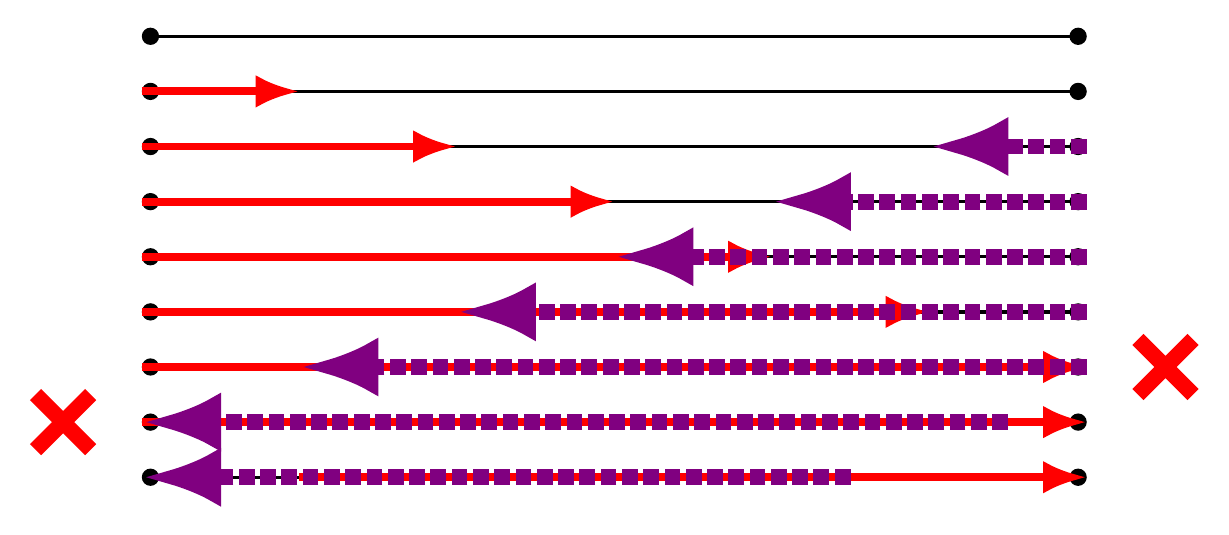
\begin{tikzpicture}[y=0.7cm]
\tikzset{
    wire/.style={draw,very thick,Circle-Circle},
    signal1/.style={draw,line width=1mm,red,-Latex},
    signal2/.style={draw,line width=2mm,dotted,violet,-Latex},
}
\draw[wire] (0, 0) -- (12, 0);
\draw[wire] (0, -1) -- (12, -1);
\draw[signal1] (0, -1) -- (2, -1);

\draw[wire] (0, -2) -- (12, -2);
\draw[signal1] (0, -2) -- (4, -2);
\draw[signal2] (12, -2) -- (10, -2);

\draw[wire] (0, -3) -- (12, -3);
\draw[signal1] (0, -3) -- (6, -3);
\draw[signal2] (12, -3) -- (8, -3);

\draw[wire] (0, -4) -- (12, -4);
\draw[signal1] (0, -4) -- (8, -4);
\draw[signal2] (12, -4) -- (6, -4);

\draw[wire] (0, -5) -- (12, -5);
\draw[signal1] (0, -5) -- (10, -5);
\draw[signal2] (12, -5) -- (4, -5);

\draw[wire] (0, -6) -- (12, -6);
\draw[signal1] (0, -6) -- (12, -6);
\draw[signal2] (12, -6) -- (2, -6);
\node[draw=red,line width=2mm,minimum width=.5cm,minimum height=.5cm,cross out] at (13, -6) {};

\draw[wire] (0, -7) -- (12, -7);
\draw[signal1] (0, -7) -- (12, -7);
\draw[signal2] (11, -7) -- (0, -7);
\node[draw=red,line width=2mm,minimum width=.5cm,minimum height=.5cm,cross out] at (-1, -7) {};

\draw[wire] (0, -8) -- (12, -8);
\draw[signal1] (2, -8) -- (12, -8);
\draw[signal2] (9, -8) -- (0, -8);
\end{tikzpicture}
\end{frame}
